\documentclass{DIKU-report}

\setlength{\errorcontextlines}{999} %Can be used for debugging purposes
\usepackage[makeindex]{imakeidx}
\usepackage{amsmath}
\usepackage{color}
\usepackage{graphicx}   
\usepackage{hyperref}
\usepackage{longtable}
\usepackage[utf8]{inputenc}
\usepackage{url}

\newcommand{\Code}[1]{\mbox{\color{blue}\texttt{#1}}}
\newcommand{\twodots}{\,.\,.\,}

\usepackage{listings,lstmisc}

\lstdefinestyle{customC++}{
  breaklines=true,
  basewidth={0.5em,0.45em},
  basicstyle=\small,
  identifierstyle=\ttfamily,
  commentstyle=\itshape,
  aboveskip=0.5 \baselineskip,
  belowskip=0.0 \baselineskip,
  xleftmargin=12pt,
  language=C++,
  numbers=left, 
  numberstyle=\tiny, 
  stepnumber=1, 
  numbersep=5pt,
  tabsize=2,
  morekeywords={constexpr,define,defined,endif,elif,ifdef,ifndef,include,noexcept,nullptr},
  keywordstyle=\bfseries,
}
\lstset{mathescape} % Allow escaping to LaTeX inside $..$
\lstset{literate=*
  {!}{{$\mbox{\textbf{not}}$}}3
}

\lstset{literate=
  {-}{{\texttt{-}}}1 
  {+}{{\texttt{+}}}1 
  {--}{{\texttt{-}\hspace*{0.05em}\texttt{-}}}2 
  {++}{{\texttt{+}\texttt{+}}}2
  {=}{{\texttt{=}}}1
  {+=}{{\texttt{+}\texttt{=}}}2 
  {-=}{{\texttt{-}\hspace*{0.05em}\texttt{=}}}2 
%  {&}{{\texttt{\&}}}1
  {[]}{{\texttt{[}$\,$\texttt{]}}}2
  {\#}{\# }2
  {\%}{\% }2
  {infty}{$\infty$}1
  {©}{\copyright{}}1 
  {§}{\textit{\S}$\!$}1 
  {ø}{{{\o}}$\!$}1 
  {ä}{{{\"a}}$\!$}1
  {^2}{${}^{2}$}1 
  {.}{{$\mathrm{\textbf{.}}\hspace*{0.05em}$}}{1}
  {->}{{$\rightarrow$}}2
  {"}{\texttt{"}}1 
  {~}{$\sim$}{2}
  {|}{{$\mid$}}1     
%  {&}{$\mathtt{\&}\!$}2
  {&}{{$\boldsymbol{\&}$}}2
  {&&}{{\hspace*{0.1em}$\boldsymbol{\&}\boldsymbol{\&}$}}3
  {()}{{$(\,)$}}2
  {==}{{$=\!=$}}2
  {!=}{{$=\!\!\!\neq\!\!\!=$}}2
  { || }{$\,\,\mbox{\textbf{or}}\,\,$}2
  {>=}{$\geq$}1
  {<=}{$\leq$}1
  {>>=}{$>$$>$\,\,$=$}3
  {---}{{\rm ---}}2
  {ell}{{$\ell$}}1
}
\lstset{style=customC++}

\titlehead{Multiplication Benchmark}
\authorhead{\{Marius-Florin Cristian; Sidharth Singhal\}}

\title{Multiplication Horse-Race}

\author{Marius-Florin Cristian; Sidharth Singhal}
 
\institute{%
Department of Computer Science, University of Copenhagen\\
Universitetsparken 5, 2100 Copenhagen East, Denmark\\ 
\texttt{wdx186@alumni.ku.dk; thx889@alumni.ku.dk}}

\begin{document}

\begin{titlepage}

\maketitle

\begin{abstract}
This progress report contains the implementation and benchmarks for different multiplication algorithms (naive, naive-encoded and karatsuba).   
\end{abstract}

\begin{keywords}
Multiplication, naive, encoded, Karatsuba, large numbers
\end{keywords}

\dates{ 2017, October 2017.}

\end{titlepage}
\tableofcontents
\subsection*{Naive and Naive-encoded Multiplication}
\subsection*{Karatsuba Multiplication}
\subsection*{Goals of experiment}
\subsection*{Approach}
\subsection*{Measures}
\subsection*{Factors and Sampling Points}
\subsection*{Generation of input (test data)}
\subsection*{Results}
\subsection*{Conclusion}
\subsection*{Future Work}
\newpage
\section{Naive and Naive-encoded Multiplication}
The naive multiplication stores each digit in an $int$, and performs the school book $O(n^2)$ digit multiplications on $std::vector<std::<vector<int>>$ (it was easier to use a matrix apparently).\\
The naive-encoded algorithm, stores one base 10 digit in a nibble, and 4 digits in a $uint16\_t$. The file $mul\_optimisation1.cpp$ exposes all of the low level helper functions, that deal with "cells" (group of 4 digits) and implements, addition, substraction, and naive multiplication at cell level. There is a higher level method called $mul\_1$ that does the  same thing for two vectors of $std::vector<uint16\_t>$ with respect to carry of each round. The result is built in a new $std::vector<uint16\_t>$ with the operations being done in place (vector cells are passed as refference).
\section{Karatsuba Multiplication}
Karatsuba multiplication algorithm reduces the multiplication of two n-digit numbers to at most ${\displaystyle n^{\log _{2}3}\approx n^{1.585}} n^{\log _{2}3}\approx n^{1.585}$ single-digit multiplications in general (and exactly ${\displaystyle n^{\log _{2}3}} n^{\log _{2}3}$ when n is a power of 2). It is therefore faster than the classical algorithm, which requires $n^2$ single-digit products.
\\Using Karatsuba's algorithm one can find the result of multiplication of two large numbers $x$ and $y$ using three multiplications of smaller numbers, each with about half as many digits as $x$ or $y$, plus some additions and digit shifts.



\section{Goals of experiment}
a) Comparison of algorithms: Benchmarking multiplication algorithms: naive and karatsuba.
\\b) Comparison of data structures: We discuss about two implementations of naive algorithm. They differ in the choice of data structure used to store a digit. The first one uses an integer to store a digit. This makes it easy to implement the algorithm. We try to improve the performance, both in terms of memory and speed, by using uint16\_t to store 4 digits, i.e., two digits per byte. 
\\c) Newsworthiness of experiment: Is it worth the extra effort of using uint16\_t?

\section{Approach}
In our initial approach, we tried to work with the metaprogramming template provided, but we failed to cast data types from $Z<n>$ to $Z<m>$;\\
Therefore, we had a change of direction and switched to an approach similar to python. The inputs are treated as strings and they are taken at run time.\\
The first problem we encountered was efficiently storing the result in memory; we initially chose a $std::vector<int>$ to build our result, where one cell represents one digit. The major drawback is obvious as one digit can have values from 0 to 9; thus occupying at most 4 bits. Thus our results were capped at around 8000 digits output before running out of memory.\\
To overcome this problem, we chose to encode our one base 10 digit on a nibble; and to store 2 digits on an unsigned char. The problem is that $char$ data type does not support multiplication. Thus we used $uint16\_t$ data structure to store 4 digits (4 nibbles). The drawback of this approach is, that on 4 bits we can represent values up to 15, and we only represent up to 9.\\
\\
By using this encoding, we expected our result to store more digits. However, the output was still capped at 8000 digits. But, there is a significant improvement in time. Further tuning can be made; as on 8 bits we store values up to 99 instead of 256.\\
\\Naive-encoded performs better than naive multiplication. Therefore, we also compare naive-encoded with the Karatsuba algorithm. Karatsuba algorithm uses the naive approach and stores the one digit in a $char$. It performs better as it uses less multiplications. 

\section{Measures}
1. CPU running time:
\\CPU running time is too small even for multiplication of large numbers. Because the system clock’s granularity cannot be chosen arbitrarily, we get distorted results. Therefore, we do several runs with the same input data,i.e., we do several runs of multiplying same numbers and report the total time taken by them.
\\2. Space consumption: 
\\We make use of as much memory as possible.
\\3. Representative operation counts:
\\The number of times helper functions(like, addition and subtraction) are called is proportional to the number of digits. For, a single call their time complexity don't make any significant change. 
\\\texttt{Naive-encoded}: The real bottleneck is the number of multiplications of type $uint16\_t$ digits.

Scalability: Handling large input numbers. The number of digits in the result are capped at 8000. This is the extent of the algorithms for our machines.

\section{Factors and Sampling Points}
Number of digits is the only factor that we change in our experiment.

\section{Generation of input numbers (test data)}
We pass number of digits as a parameter to the function which computes a random number. We use \texttt{uniform\_int\_distribution} from std library to generate every digit independently. The random number engine is used from \texttt{mt199337} from std library.
\\Time taken to generate the numbers is not taken into consideration.
\section{System Info}
\lstinputlisting[caption=Machine 1,label=dmi_proc_m1,language=,]{listings/dmidecode_processor}
\vspace*{\fill}
\newpage
\section{Results}
\begin{figure}[h]
\makebox[\textwidth]{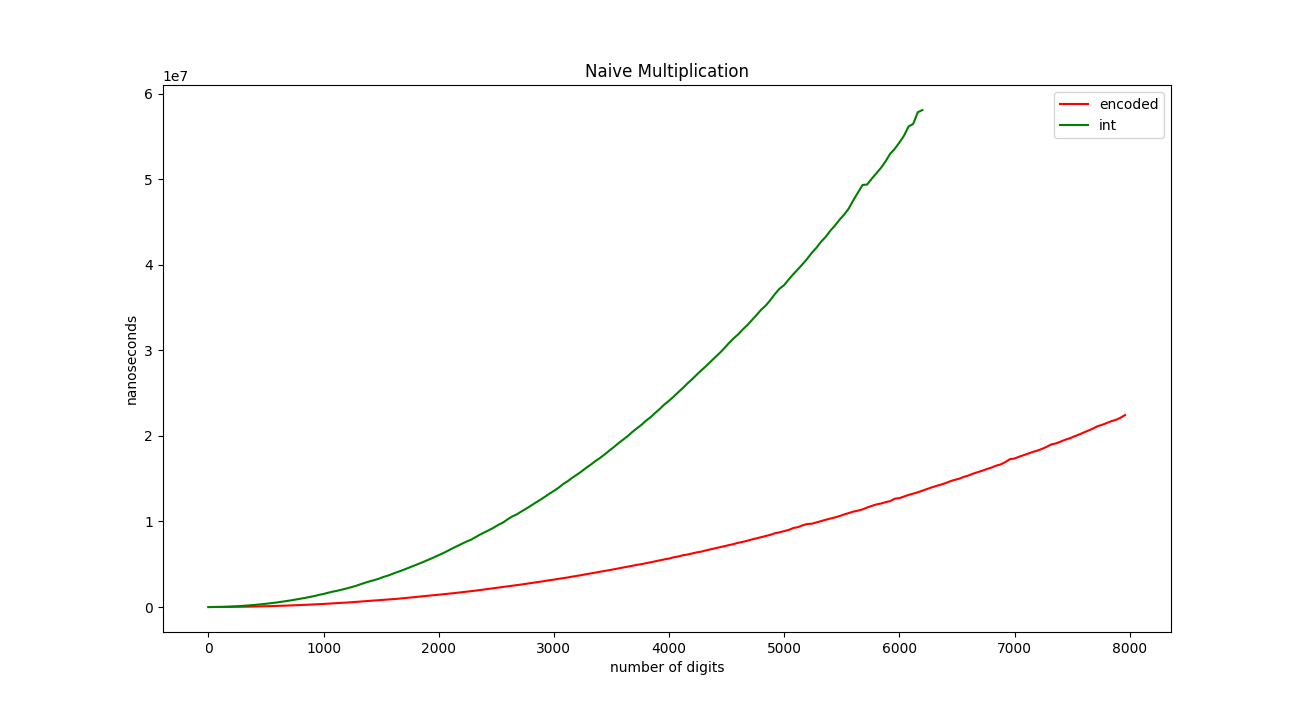
\includegraphics[width=\paperwidth]{naive_v_encoded}}
\end{figure}
\begin{figure}[h]
\makebox[\textwidth]{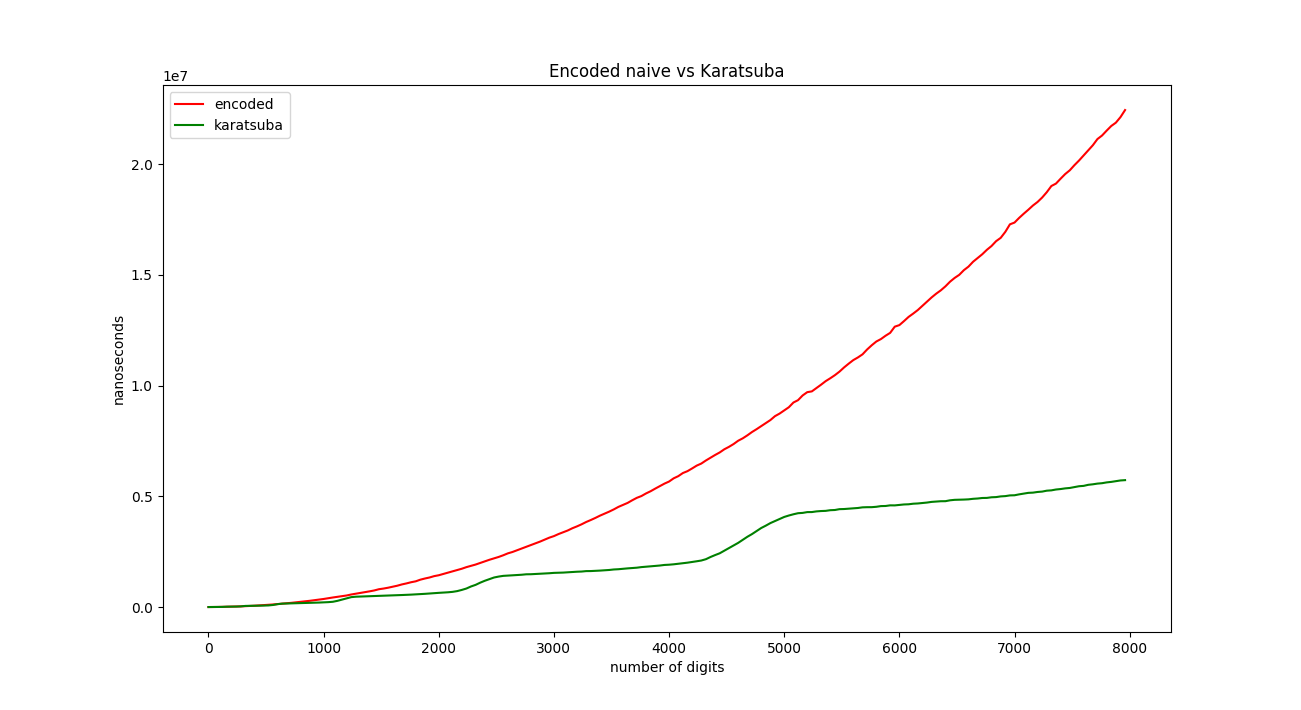
\includegraphics[width=\paperwidth]{enc_v_karatsuba}}
\end{figure}
\vspace*{\fill}
\newpage
\section{Conclusion}
As expected Karatsuba is performing better; But we are still capped at the number of digits. The encoded version does not help in increasing the number of digits, but improves the time complexity. 
\section{Future Work}
1. Karatsuba: Implementation of Karatsuba using the encoded format. 
2. Instead of having cell size of $uint16\_t$ we can use $long\ long$. Will this result in an improvement on the amount of digits we can use?\\
3. Why not have a lookup table for cell multiplication values, and do it in O(1); this table will take up memory space, it might make it faster for instances up to a number of digits, but the trade off will be in the length of the result.\\
4. $x^{z}$ is computed much faster than $x_1x_2...x_z$ (exponentiation by squaring); having a lookup table to break the cell in power of primes, will this yield in better performance?

\bibliographystyle{DIKU}
%\begin{thebibliography}{techreport}
%hey
%\end{thebibliography}
%
%\begin{bibliography}{1}

%\bibitem{recent} FAST INTEGER MULTIPLICATION USING GENERALIZED FERMAT PRIMES - SVYATOSLAV COVANOV AND EMMANUEL THOMÉ \url{https://arxiv.org/pdf/1502.02800.pdf}

%\end{bibliography}
\end{document}
